\chapter{NC Experiment 1}

% DONE
\section{Design}
\paragraph{}The purpose of the first experiment was to compare the NC to WDRC using a realistic sample of WDRC hearing aids.  Thus, we decided to recruit participants who currently wore WDRC hearing aids, and lent out a set of NC hearing aids for each participant to wear.

Figure 4.1 shows a week by week schematic of the study design.  At the very beginning of the study, participants were issued a freeform diary, and were encouraged to describe their experiences of various sounds in their everyday environments.  Specifically, they were asked to take note of any unusual sounds, any instances of feedback, and whether any sounds were too loud or too quiet.  Half of the participants were randomly assigned to begin the study wearing their own WDRC hearing aids, while the other half were fit with NC hearing aids.  After a two week period of wearing the hearing aids (deemed the first adaptation period), if a participant started out with NCs, they were given an adjustment to the NCs by a trained hearing instrument specialist (HIS).  After the NCs had been adjusted, participants wore the hearing aids for another two weeks (the second adaptation period) before coming in for two, two hour test sessions, spaced one week apart.  Otherwise, if a participant was assigned to wear WDRC hearing aids first, they waited two weeks before coming in for the two, two hour test sessions.

\begin{figure}[htp]
\begin{center}
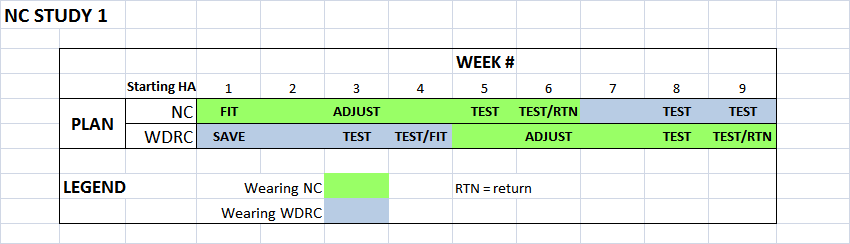
\includegraphics[width=\textwidth]{chap4-design.png}\\
\caption[NCStudy1 design]{NCStudy1 design.  Half of the participants started the study wearing WDRC hearing aids, while the other half were fit with NCs at the outset.  Adjustments were only given to the NCs, as the participants did not require adjustments to their own set of WDRC hearing aids, which they had already adapted to over months and years of wearing them.  Halfway through the study, participants began wearing the second set of hearing aids.  Two test sessions were conducted for each pair of hearing aids.}
\label{ch4-design}
\end{center}
\end{figure}

Adjustments were guided by observations that participants had recorded in their diaries, as well as from verbal reports given by the participant at the time of the adjustment.  Following the second test session, participants who first wore NCs returned the set of NCs, and participants who first wore WDRC were given a set of NCs which had been preprogrammed to fit their loss.

\section{Participants}
% DONE
\subsection{Demographics and Prior Experience}
\paragraph{}A total of 8 participants qualified for the study (3 male, 5 female), with an average age of 76 (SD = 7.7).  All participants had prior experience wearing hearing aids for several years, and spoke English as their primary language.  The hearing aids that participants wore coming into the study were from assorted manufacturers (Oticon, Phonak, Siemens), and were in different styles (mostly behind-the-ear (BTE) or receiver-in-the-canal (RIC); 2 participants wore in-the-canal styles (ITC)).  The average age of the WDRC hearing aids being worn in the study was 3 years (SD = 2).

% DONE
\subsection{Audiograms}
\paragraph{}Prior to their inclusion in the study, participants visited McMaster University for a hearing test; air conduction thresholds for both ears and bone conduction thresholds for the worse ear were measured.  A trained student performed the measurements, following the British Society of Audiology recommended procedure for pure-tone audiometry \cite{BSA2004} as closely as possible.

To qualify for the study, participants were required to have symmetrical sensorineural hearing loss and currently wear 2 hearing aids.  More specifically, participants were included on the basis of the following criteria: 1) no difference greater than 10 dB HL between ears on the calculated pure tone average (PTA; the average of 0.5, 1, and 2 kHz), 2) no difference greater than 30 dB HL at any audiometric frequency between the two ears, and 3) no difference greater than 15 dB HL between air conduction and bone conduction thresholds at any audiometric frequency.  Due to the limited supply of subjects, one participant was included who had an asymmetrical hearing loss, according to our definition.

After qualifying for inclusion in the study, the first session required participants to visit McMaster University, in order for the HIS to hook up their existing hearing aids so that their old audiogram data could be read and extracted.  If they were assigned to wear NC hearing aids first, they were given a pair of NCs at the end of the session.  The purpose of collecting the old audiogram data was to allow for a fair comparison between the NC and WDRC.  Hearing loss changes over time, and several of the participants had not had their hearing retested or their hearing aids adjusted for months, and in some cases, years.  Thus, programming the NCs using a newer, fresher audiogram, would have introduced a bias in favor of the NC.  For two participants, we were unable to read the old audiogram data programmed on their existing hearing aids, and thus had no choice but to use the new audiogram data to program the NCs.  Figure 4.2 plots both the new and the old audiogram data for each participant.

\begin{figure}[htp]
\begin{center}
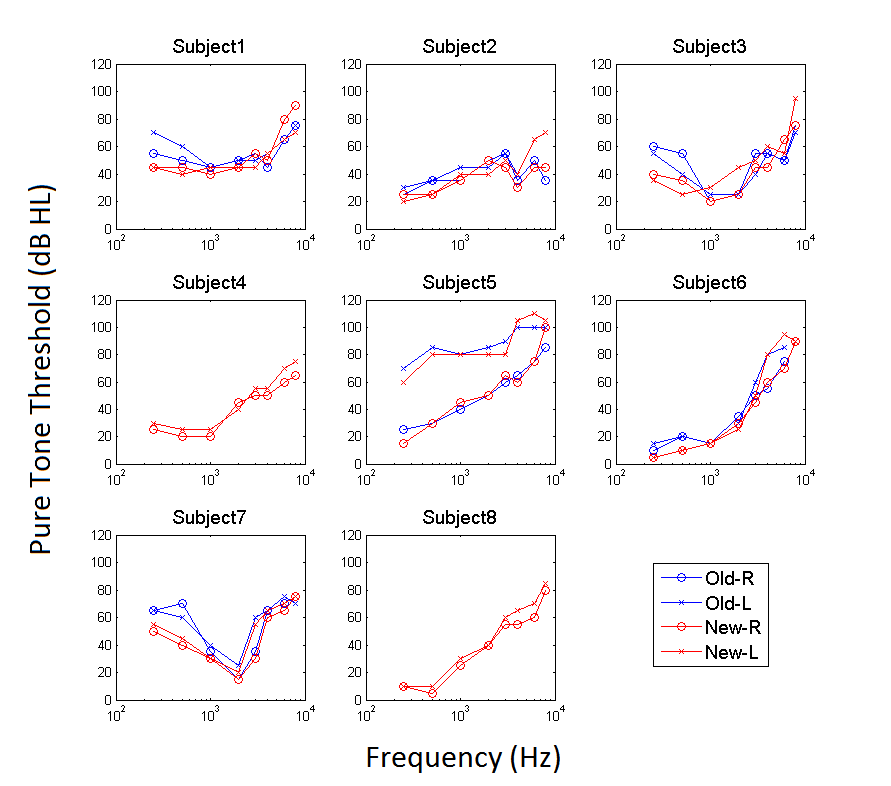
\includegraphics[width=\textwidth]{chap4-audiograms.png}\\
\caption[NCStudy1 old and new audiograms for all subjects]{Old and new audiograms for all subjects.  New audiograms are plotted in red, old audiograms in blue, x's denote measurements obtained for the left ear, and o's denote measurements obtained for the right ear.  For the most part, the new and old audiograms matched quite closely.  Subject 5 had an asymmetrical hearing loss.  The HIS was unable to read audiogram data from subjects 4 and 8 due to software incompatibilities with their devices.}
\label{ch4-audiograms}
\end{center}
\end{figure}

% DONE
\subsection{Subjects Analyzed}
\paragraph{}Despite initially recruiting 8 subjects, only 5 subjects were suitable for data analysis (subjects 2, 3, 4, 7, and 8).  Subject 1 was removed from data analysis because he/she was unable to complete a few of the tasks.  Subject 5 was removed from analysis because of the asymmetrical nature of his/her hearing loss.  Subject 6 dropped out of the study after a few weeks of participation, so his/her dataset was incomplete.

% NEED SOME TECHNICAL DETAILS
\section{Testing Room and General Procedures}
\paragraph{}The two hour test sessions were conducted in a sound attenuating chamber.  For all of the experiments, stimuli were either prerecorded or generated using Matlab (exception: the HINT was programmed with Visual Basic 6).  Stimuli were presented through two Tucker-Davis-Technologies Programmable Attenuators (TDT PA5s; one for the left channel and one for the right channel), routed through a TDT Signal Mixer (TDT SM5) to create a mono signal, amplified with a Hafler P1000 Trans.Ana 110 watt amp, and subsequently routed to the appropriate loudspeaker using a TDT RV8 and PM2.  There were 7 speakers (Audio Video Methods P73), arranged in a 90$^\circ$ arc for the purpose of testing sound localization.  All of the other experiments used only one speaker, located directly in front of the participant (0$^\circ$ azimuth).

All SPL measurements were performed with a Bruel \& Kjaer 2239A sound level meter located at the centre of where the participant's head would be located in space.  To ensure consistency in the participant's location in the room, tape markings were made on the floor, and a table rested within these tape markings.  For the hVd, VCV, mistuned harmonic, timbre perception, and gap detection experiments, participants responded using a touchscreen (Planar PT1510MX), which was propped up on the table in a consistent location.  For the other experiments (sound localization, HINT), the experimenter rested the touchscreen in his/her lap.  Participants sat 1.5 meters away from the speakers, with their ears level with the centre of the speaker cones (cone diameter of 17 cm).  Figure 4.3 shows the room setup for the sound localization experiment.

\begin{figure}[htp]
\begin{center}
\includegraphics[width=\textwidth]{chap4-sound-booth.png} \\
\caption[Sound attenuating chamber - experimental setup]{Sound attenuating chamber - experimental setup.  With the exception of the sound localization experiment, participants faced speaker A for all experiments.}
\label{ch4-sound-booth}
\end{center}
\end{figure}

In the following sections, stimuli, procedures, and results will be presented one by one for each task, organized by auditory domain (speech intelligibility, music perception, sound localization, subjective measures).  Analyses for all experiments were performed in R \cite{R2013}.  Where appropriate, the Huynh-Feldt correction for deviations from sphericity ($\tilde{\epsilon}$) was used to compute p values from F tests on within-subjects factors \cite{Maxwell2004}.  In data tables, degrees of freedom and sums of squares for both the numerator (effect of interest) and denominator (error) are reported, along with F and p values, and a measure of effect size, generalized eta squared (abbreviated \emph{ges}).

\section{Speech Intelligibility}
\subsection{Hearing In Noise Test (HINT)}
\subsubsection{Procedure}
\paragraph{}Participants sat in a sound attenuating chamber facing the speaker at a 0 $^\circ$ azimuth.  The SSN was measured to be 65 dB(A), and this presentation level remained constant during the course of the experiment.  For each session (one for each set of hearing aids), 2 lists of sentences were used, taking care not to use the same lists in the second session as the first session.  The presentation level of the first sentence was initially attenuated such that its presentation level was 10 dB less than the noise, and was increased by 4 dB until it was recognized correctly by the participant, at which point it was decreased by 4 dB.  For the next 3 sentences, if the participant correctly (incorrectly) recognized the sentence, the sentence presentation level was decreased (increased) by 4 dB.  Similarly, the presentation level of each of the remaining 16 sentences was adaptively adjusted based on whether the previous response was correct or incorrect, but instead a 2 dB step was used.  To obtain a SRT measurement for a participant (SNR at 50\% correct), the presentation levels of the fifth sentence to the twentieth sentence, including the level of a would-be twenty-first sentence, were averaged.  The SNR was computed by subtracting the noise level from the average sentence presentation level.
\subsubsection{Results}
\paragraph{}A within-subjects ANOVA with a 2-level factor (hearing aid) was performed, with SRT as the dependent measure.  There was no significant effect of hearing aid (F(1,4) = 0.42, p = 0.551).  Group means and standard errors are plotted in Figure 4.4, and individual SRT means and standard deviations are plotted in Figure 4.5.  Individual differences in speech intelligibility in noise were far greater than any difference between the two hearing aids.

\begin{figure}[htp]
\begin{center}
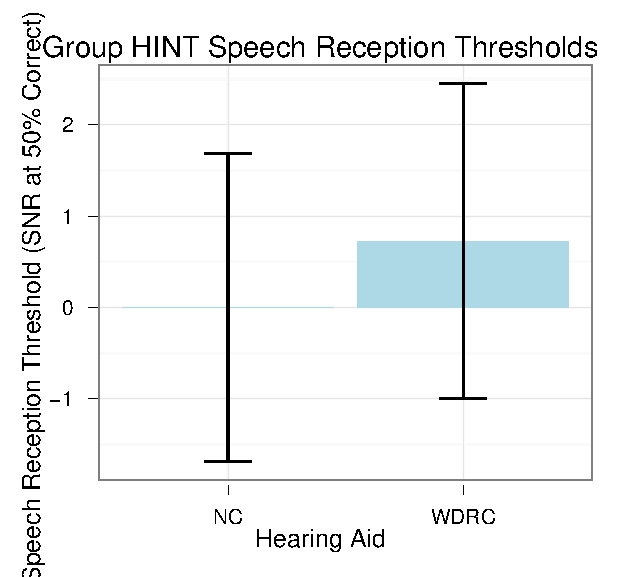
\includegraphics[height=3in]{chap4-hint-group.pdf} \\
\caption[NCStudy1 group results on the HINT]{NCStudy1 group results on the HINT.  Error bars represent $\pm$ 1 SEM.  Speech reception thresholds were calculated by subtracting the noise level from the average presentation level of the last 16 sentences presented.  There was no significant difference in performance between NC and WDRC (F(1,4) = 0.42, p = 0.551).}
\label{ch4-hint-group}
\end{center}
\end{figure}

\begin{figure}[htp]
\begin{center}
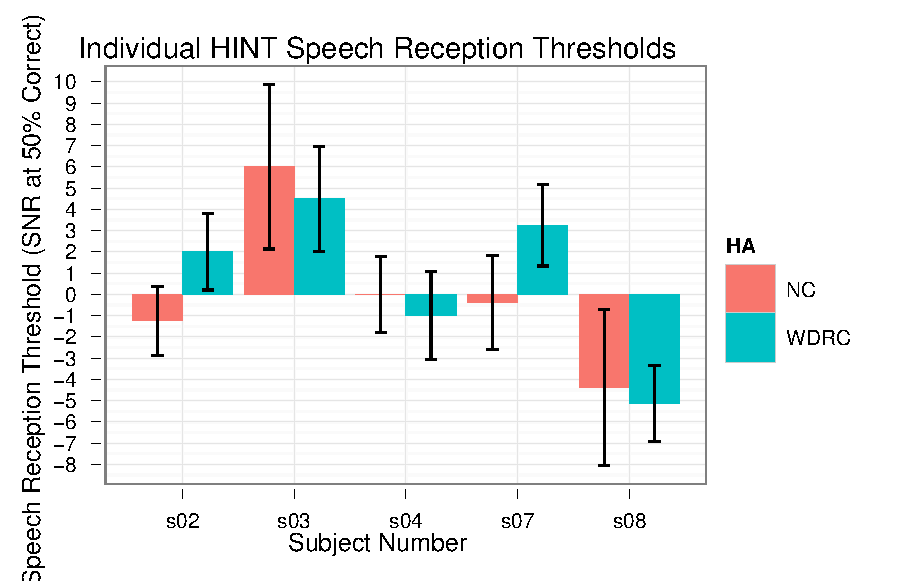
\includegraphics[height=3in]{chap4-hint-indiv.pdf} \\
\caption[NCStudy1 individual results on the HINT]{NCStudy1 individual results on the HINT.  Error bars represent $\pm$ 1 SD.  Speech reception thresholds were calculated by subtracting the noise level from the average presentation level of the last 16 sentences presented.  Most participants performed approximately equally between the NC and WDRC, however, subjects 02 and 07 performed considerably better with the NC.}
\label{ch4-hint-indiv}
\end{center}
\end{figure}

\subsection{Consonant Vowel Consonant (CVC)}
\subsubsection{Stimuli}
\paragraph{}CVC stimuli were extracted from the \citeA{Hillenbrand1995} corpus, which contains 12 vowel sounds (/i, \textsci , $\varepsilon$, \ae , \textscripta , \textopeno , \textscu , u, \textturnv , \textrhookrevepsilon , e, o/) in hVd syllables spoken by 45 men, 48 women, and 46 children.  All stimuli were normalized to the same root-mean square level.  We selected 10 talkers in total (5 men, 5 women) and 11 hVd pronunciations for a total of 110 CVC tokens (10 talkers * 11 syllables).  /hod/ was removed from the test set, since it sounded too similar to /hawed/ and could have resulted in ambiguity in the analysis of responses.

Multi-talker babble was used as a noise condition that featured 100 talkers in a cafeteria.  The babble was downsampled from its original sampling rate to 16000 Hz to match the sampling rate of the Hillenbrand et al. stimuli.
\subsubsection{Procedure}
\paragraph{}This task took approximately 25 minutes to complete.  The participant sat in the sound attenuating chamber and listened to CVC stimuli either in quiet or embedded in multi-talker babble, presented through the speaker at a 0$^\circ$ azimuth.

The CVC tokens had an average presentation level of 67.5 dB(A), and for the noise condition, the noise level was set to 62.5 dB(A).  In the noise condition, a 2000 ms clip of noise was randomly selected from the multi-talker babble source on each trial, and the CVC stimulus began anywhere in the range of 600 ms to 1000 ms after noise onset, with equal probability (rectangular distribution).  The noise sample was cosine windowed with a rise and fall of 100 ms.  Following stimulus delivery on a given trial, the participant pressed on the word they heard (had, hawed, hayed, head, heard, heed, hid, hoed, hood, who'd, hud) using the touchscreen.  After responding, there was a 1000 ms period of silence before the next trial began.  Feedback was not given on correct or incorrect responses.

There were a total of 5 blocks, each containing 2 presentations of each word in both quiet and noise, resulting in 44 presentations per block (2 talkers * 2 conditions * 11 words), and a grand total of 220 trials for the whole experiment.  The presentation order was completely random within a block, and all CVC tokens were used twice (once for quiet, once for noise).

There was no training session, although prior to beginning the experiment, the experimenter asked the participant to read the words on the touchscreen out loud.  If one of the tokens was pronounced incorrectly, the experimenter verbalized the correct pronunciation and asked the participant to repeat it.  Breaks between blocks were self-paced.
\subsubsection{Results}
\paragraph{}A within-subjects ANOVA was performed, with two within-subjects factors, hearing aid (WDRC or NC), and condition (quiet or noise).  The dependent measure was the percentage of hVd tokens correctly identified.  The only significant effect was condition (F(1,4) = 19.23, p = 0.011), such that the noise condition was more difficult than the quiet condition.  Detailed statistical results may be seen in Table 4.1.  Group means and standard errors are plotted in Figure 4.6, and individual means are plotted in Figure 4.7.

\begin{table}[htp]
\begin{center}
\begin{tabular}{lrrrrrrrr}
       Effect & DFn & DFd  &  SSn &  SSd  &    F  &     p & p<.05  &   ges \\
       \hline
          HA  & 1  & 4 & 1.5 &  18.8 &  0.32 & 0.603   &    & 0.001 \\
        cond  & 1 &  4 & 464.0  &  96.4 & 19.23 & 0.011 &    * & 0.241 \\
     HA:cond  & 1  & 4 & 4.1 &  26.9 &  0.62 & 0.477   &    & 0.003 \\
     \hline
\end{tabular}
\end{center}
\caption{hVd Within-Subjects ANOVA}
\end{table}

\begin{figure}[htp]
\begin{center}
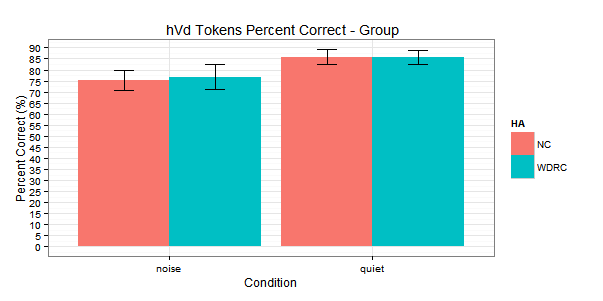
\includegraphics[height=3in]{chap4-hVd-group.png} \\
\caption[NCStudy1 hVd token percent correct - group]{NCStudy1 hVd token percent correct - group.  Error bars represent $\pm$ 1 SEM.  There was no significant difference in performance between NC and WDRC on the percentage of hVd tokens correctly identified (F(1,4) = 0.32, p = 0.603).}
\label{ch4-hVd-group}
\end{center}
\end{figure}

\begin{figure}[htp]
\begin{center}
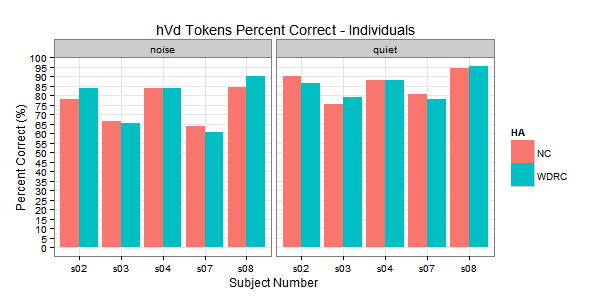
\includegraphics[height=3in]{chap4-hVd-indiv.png} \\
\caption[NCStudy1 hVd token percent correct - individuals]{NCStudy1 hVd token percent correct - individuals.  Some participants correctly identified more hVd tokens with WDRC, while others performed better with NC.}
\label{ch4-hVd-indiv}
\end{center}
\end{figure}

Although there were no significant differences between hearing aids on the overall percentage of hVd tokens correctly identified, there were fairly consistent differences between the hearing aids on individual phonemes.  Figure 4.8 plots a confusion matrix both for NC and WDRC averaged over both noise conditions, to illustrate the difficulty of individual phonemes in the experiment.  Each value in the confusion matrix is the percentage of times responding with a given response, given the stimulus that was presented.  Adding all values across a single row will total 100\%, to within rounding error.  Figure 4.9 plots the difference between the NC and WDRC confusion matrices separately for both the quiet and noise conditions.

\begin{figure}[htp]
\begin{center}
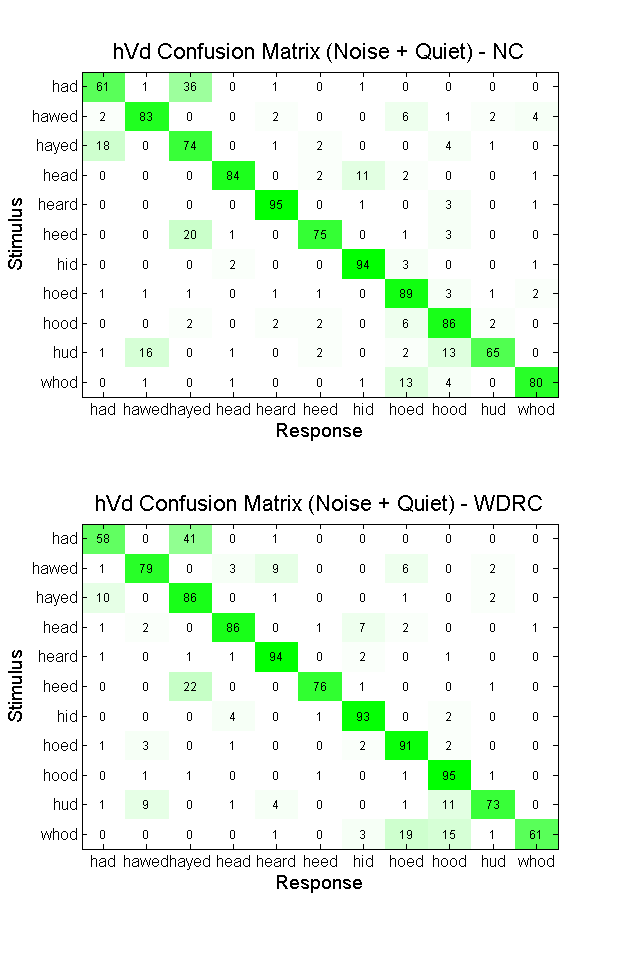
\includegraphics[height=7in]{chap4-hVd-ovr.png} \\
\caption[NCStudy1 hVd overall confusion matrices]{NCStudy1 hVd overall confusion matrices.  Data shown are for the noise and quiet conditions amalgamated together.  \emph{Top}: hVd confusion matrix for NC.  \emph{Bottom}: hVd confusion matrix for WDRC.  For many of the syllables, performance is at near ceiling.  Few differences exist between NC and WDRC; the words where WDRC and NC differ the most are /hayed/, /hood/, /hud/, and /who'd/. }
\label{ch4-hVd-ovr}
\end{center}
\end{figure}

\begin{figure}[htp]
\begin{center}
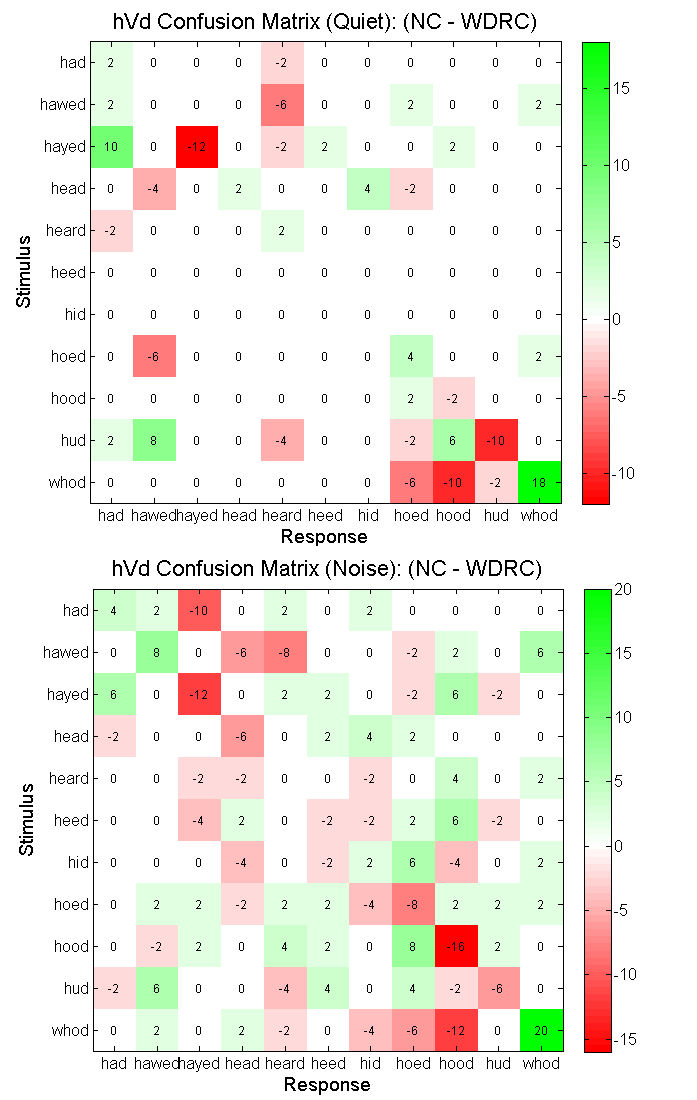
\includegraphics[height=7in]{chap4-hVd-cond-difference.png} \\
\caption[NCStudy1 difference between hVd confusion matrices (NC - WDRC)]{NCStudy1 difference between hVd confusion matrices (NC - WDRC).  \emph{Top:} Difference between hVd confusion matrices for the quiet condition.  \emph{Bottom:} Difference between hVd confusion matrices for the noise condition.  Each tile represents NC \% response - WDRC \% response.  In quiet, NC seems to restore /who'd/ better than WDRC, while WDRC favors /hayed/ and /hud/.  In noise, NC restores /who'd/ better than WDRC, while WDRC restores /hayed/ and /hood/ better.}
\label{ch4-hVd-cond-diff}
\end{center}
\end{figure}

\subsection{Vowel Consonant Vowel (VCV)}
\subsubsection{Stimuli}
\paragraph{}The stimuli used for the VCV experiment were extracted from the training set found in The Interspeech 2008 Consonant Challenge \cite{Cooke2008}.  The VCV stimuli contained in this corpus were professionally recorded by trained British talkers with no strong regional accents, and normalized to the same root-mean square level.  For our experiment, we selected 6 talkers with complete data sets (3 male, 3 female), 21 consonant sounds (/b/, /d/, /g/, /p/, /t/, /k/, /s/, /sh/, /f/, /v/, /th/, /ch/, /z/, /zh/, /h/, /m/, /n/, /w/, /r/, /y/, /l/), 1 vowel (/\ae /), 1 stress (first syllable), and 2 conditions (noise and quiet), for a grand total of 252 VCV tokens (6 talkers * 21 consonant sounds * 1 vowel * 1 stress * 2 conditions).
\subsubsection{Procedure}
\paragraph{}Similar to the CVC task, the whole procedure took approximately 25 minutes.  The participant sat in the sound attenuating chamber while VCV stimuli were presented through a loudspeaker, with the same positioning as that used in the HINT and CVC experiments.  On the table in front of the participant sat a touchscreen displaying a grid of consonants and example pronunciations, representing all possible responses the participant could choose from.  After the presentation of a VCV stimulus, the participant selected the consonant from the grid that corresponded best with the consonant that they heard.  The presentation level of the VCV nonsense syllables was fixed at 67.5 dB(A), and the noise was fixed at 62.5 dB(A).

In the noise condition, a 2000 ms clip of noise was randomly selected from the multi-talker babble source on each trial, and the CVC stimulus began anywhere in the range of 600 ms to 1000 ms after noise onset, with equal probability (rectangular distribution).  The noise sample was cosine windowed with a rise and fall of 100 ms. Following stimulus delivery on a given trial, the participant pressed on the VCV token that they heard, using the touchscreen.  After responding, there was a 1000 ms period of silence before the next trial began.  Feedback was not given on correct or incorrect responses.

There were a total of 6 blocks, each containing 1 presentation of each VCV token in both quiet and noise, resulting in 42 presentations per block (1 talker * 2 conditions * 21 words).  The presentation order was completely random within a block, and all VCV tokens were used twice (one for quiet, one for noise).

There was no training session, although prior to beginning the experiment, the experimenter asked the participant to read the words on the touchscreen out loud.  If one of the tokens was pronounced incorrectly, the experimenter verbalized the correct pronunciation and asked the participant to repeat it.
\subsubsection{Results}
\paragraph{}A within-subjects ANOVA was performed, with two within-subjects factors, hearing aid (WDRC or NC), and condition (quiet or noise).  The dependent measure was the percentage of VCV tokens correctly identified.  The only significant effect was a main effect of condition (F(1,4) = 168.62, p < 0.001), such that the noise condition was much more difficult than the quiet condition.  Detailed statistical results may be seen in Table 4.2.  Group means and standard errors are plotted in Figure 4.10, and individual means are plotted in Figure 4.11.

\begin{table}[htp]
\begin{center}
\begin{tabular}{lrrrrrrrr}
       Effect & DFn & DFd  &  SSn &  SSd  &    F  &     p & p<.05  &   ges \\
       \hline
          HA &  1 &  4 &   99.1 & 200.8 &   1.97 & 0.233 &      & 0.037 \\
        cond &  1 &  4 & 2687.0 &  63.7 & 168.62 & 0.000 &    *** & 0.509 \\
     HA:cond &  1 &  4 &    8.2 &  24.3 &   1.34 & 0.311 &      & 0.003 \\
     \hline
\end{tabular}
\end{center}
\caption{VCV Within-Subjects ANOVA}
\end{table}

\begin{figure}[htp]
\begin{center}
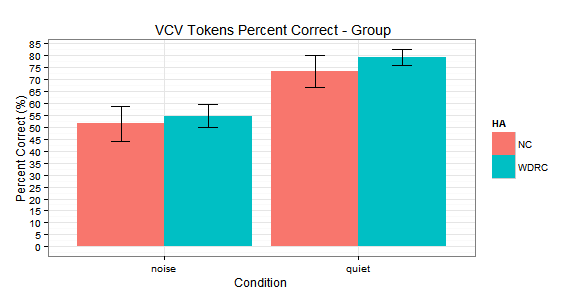
\includegraphics[height=3in]{chap4-vcv-group.png} \\
\caption[NCStudy1 VCV token percent correct - group]{NCStudy1 VCV token percent correct - group.  Error bars represent $\pm$ 1 SEM.  There was no significant difference in performance between NC and WDRC on the percentage of VCV tokens correctly identified (F(1,4) = 1.97, p = 0.233).}
\label{ch4-vcv-group}
\end{center}
\end{figure}

\begin{figure}[htp]
\begin{center}
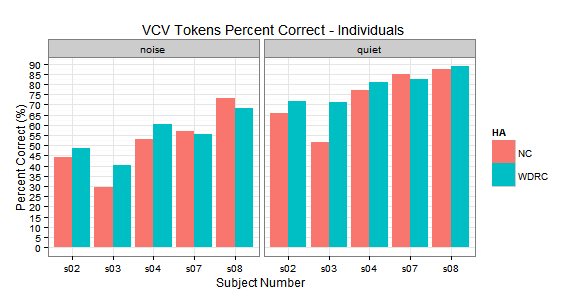
\includegraphics[height=3in]{chap4-vcv-indiv.png} \\
\caption[NCStudy1 VCV token percent correct - individuals]{NCStudy1 VCV token percent correct - individuals.  There were some individuals who performed better with WDRC (in particular, subject 03), while others did better with NC.}
\label{ch4-vcv-indiv}
\end{center}
\end{figure}

Although there were no significant differences between hearing aids on the overall percentage of VCV tokens correctly identified, there were consistent differences between the hearing aids on individual phonemes.  Figure 4.12 plots a confusion matrix both for NC and WDRC averaged over both the quiet and noise conditions, to illustrate the difficulty of individual phonemes in the experiment.  Figure 4.13 plots the difference between the NC and WDRC confusion matrices for both the quiet and noise SNR conditions.

\begin{figure}[htp]
\begin{center}
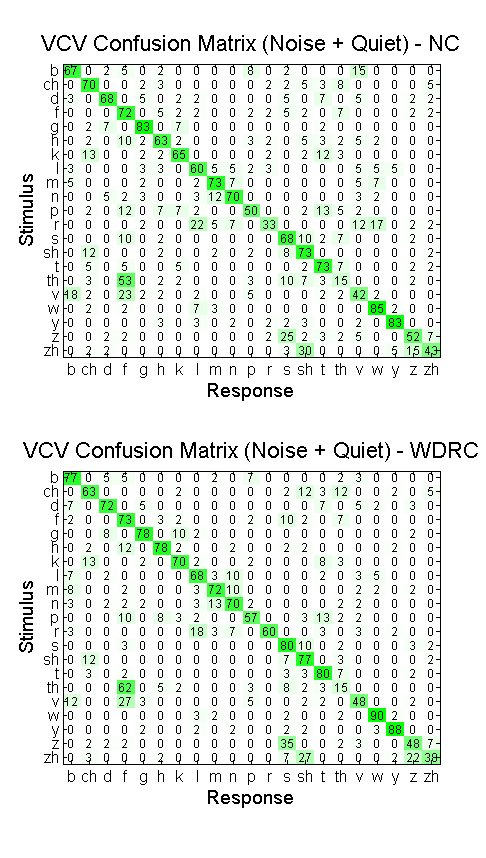
\includegraphics[height=7in]{chap4-VCV-ovr.png} \\
\caption[NCStudy1 VCV overall confusion matrices]{NCStudy1 VCV overall confusion matrices.  Data shown are for the noise and quiet conditions amalgamated together.  \emph{Top}: VCV confusion matrix for NC.  \emph{Bottom}: VCV confusion matrix for WDRC.}
\label{ch4-VCV-ovr}
\end{center}
\end{figure}

\clearpage

\begin{figure}[htp]
\begin{center}
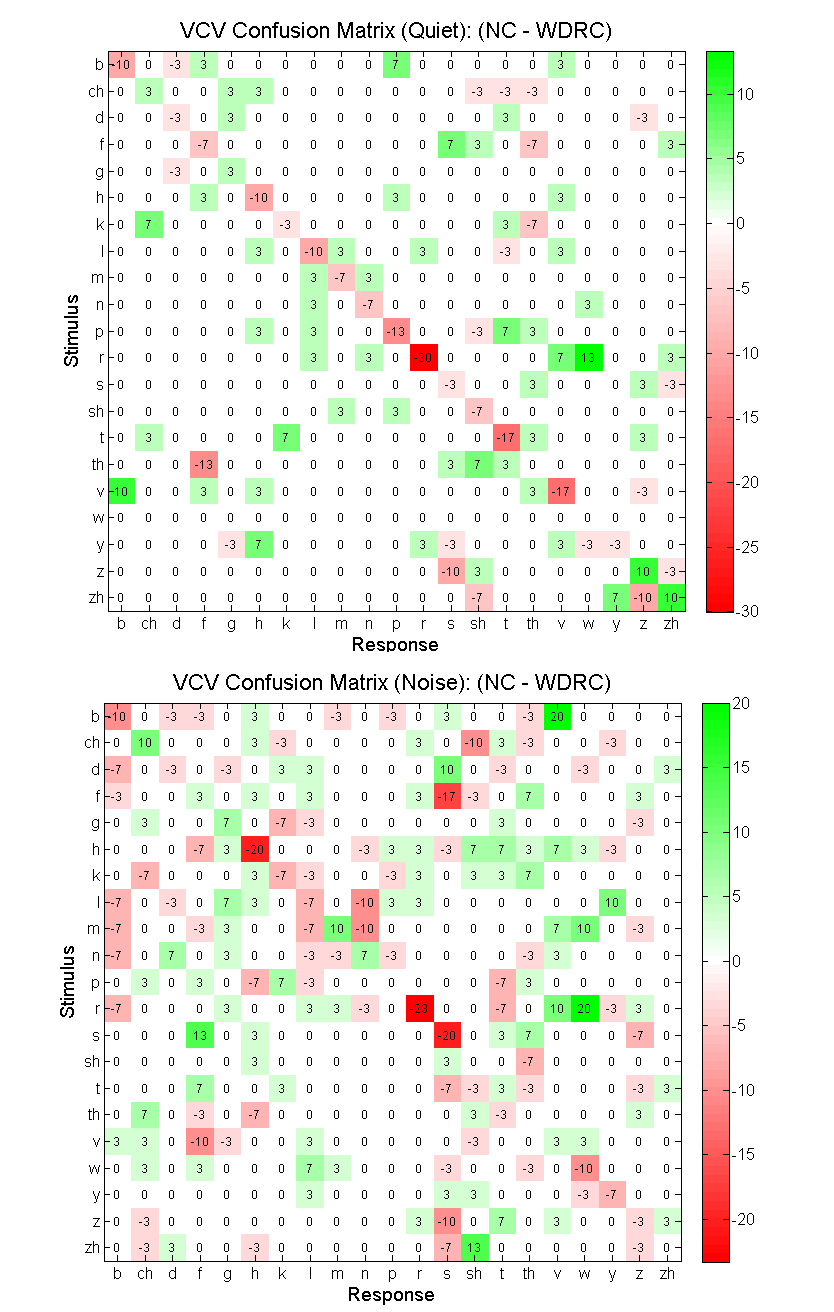
\includegraphics[height=7in]{chap4-vcv-cond-difference.png} \\
\caption[NCStudy1 difference between VCV confusion matrices (NC - WDRC) ]{NCStudy1 difference between VCV confusion matrices (NC - WDRC).  \emph{Top:} Difference between VCV confusion matrices for the quiet condition.  \emph{Bottom:} Difference between VCV confusion matrices for the noise condition.  The NC had consistent trouble with a few consonants across both the noise and quiet conditions (/b/, /h/, and /r/).}
\label{ch4-VCV-cond-diff}
\end{center}
\end{figure}


\section{Music Perception}
\subsection{Mistuned Harmonic}
\subsubsection{Stimuli}
\paragraph{}Complex tones with 10 harmonics (fundamental frequency of 200 Hz or 600 Hz) of random phase and equal intensity were created in Matlab.  The stimulus was presented at a level of 65 dB SPL measured in absence of the participant at the location of where the participant's head would be in space.  The complex tones were presented in a background of white Gaussian noise set at 55 dB(A) (resulting in a SNR of +10).  The level of the noise was decided upon by presenting the complex tones and noise to the NC to see if any feedback or entrainment could be detected by the experimenter.  Lower SNR values corresponded with less entrainment, so we selected the approximate maximum SNR which produced no audible entrainment.
\subsubsection{Procedure}
\paragraph{}A three-alternative forced-choice (3AFC) adaptive staircase design \cite{Levitt1971} with a 2-down, 1-up rule was used to estimate the mistuned harmonic threshold.  A trial consisted of 3, 500 ms presentations of a complex tone with an inter-stimulus interval (ISI) of 500 ms.  One of the 3 complex tones in a trial had the third harmonic mistuned in the upward direction, starting with a (maximum) mistuning of 30\%, and it was the task of the participant to identify ``which tone sounded different than the other two'' by selecting the corresponding button on a touchscreen.

There were 2 blocks in the experiment, and the blocks differed with respect to the fundamental frequency of the complex tone.  The first block was always the 200 Hz tone, and the second block was always the 600 Hz tone.  Each block consisted of 12 reversals (defined as a transition from at least 2 correct responses to an incorrect response, or vice versa).  The percentage mistuning was altered by a factor of 1.4 according to the 2-down, 1-up rule.  The mistuned harmonic threshold for a given block was computed by averaging the thresholds measured at the last 8 reversals in the block.

Continuous white Gaussian noise played throughout the presentation of the complex tones, including a 500 ms segment before the first complex tone and a 500 ms segment after the last complex tone.  Both the complex tones and the white Gaussian noise were cosine ramped with a linear rise/fall time of 10 ms.

Feedback on task performance (correct or incorrect) was given to participants on every trial via the touchscreen, and was displayed for 2000 ms.  Following the feedback, there was a silent period for 1000 ms preceding the onset of the next trial.  A practice session featuring 6 trials was included before the first experimental block to ensure that the participant understood the instructions.  The practice session was repeated until participants admitted that they understood the task, and until they exceeded 50\% correct on the practice trials.  For the vast majority of subjects, only 1 practice session was required.
\subsubsection{Results}
\paragraph{}A within-subjects ANOVA was performed, with two within-subjects factors, hearing aid (WDRC or NC), and tone (200 Hz or 600 Hz).  The dependent measure was the mistuned harmonic threshold, computed by averaging the last 8 reversals on each block.  There were no significant main effects or an interaction.  Detailed statistical results may be seen in Table 4.3.  Group means and standard errors are plotted in Figure 4.14, and individual means and standard deviations are plotted in Figure 4.15.

\begin{table}[htp]
\begin{center}
\begin{tabular}{lrrrrrrrr}
       Effect & DFn & DFd  &  SSn &  SSd  &    F  &     p & p<.05  &   ges \\
       \hline
          HA &  1 &  4 & 47.5 & 67.6 &  2.81 & 0.169 &   &   0.076 \\
        harm &  1  & 4 &  2.3 & 136.2 & 0.07 & 0.810 &   &   0.004 \\
     HA:harm &  1 &  4 &  8.1 & 115.9 & 0.28 & 0.623 &   &   0.014 \\
     \hline
\end{tabular}
\end{center}
\caption{Mistuned Harmonic Within-Subjects Factorial ANOVA}
\end{table}

\begin{figure}[htp]
\begin{center}
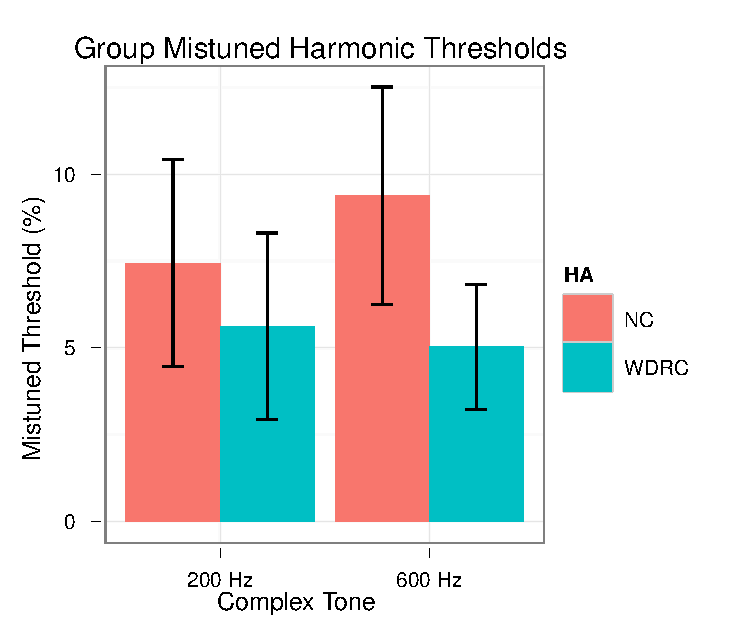
\includegraphics[height=3in]{chap4-mhn-group.pdf} \\
\caption[NCStudy1 mistuned harmonic - group thresholds]{NCStudy1 mistuned harmonic - group thresholds.  Error bars represent $\pm$ 1 SEM.  There was no significant difference between NC and WDRC (F(1,4) = 2.81, p = 0.169).}
\label{ch4-mhn-group}
\end{center}
\end{figure}

\begin{figure}[htp]
\begin{center}
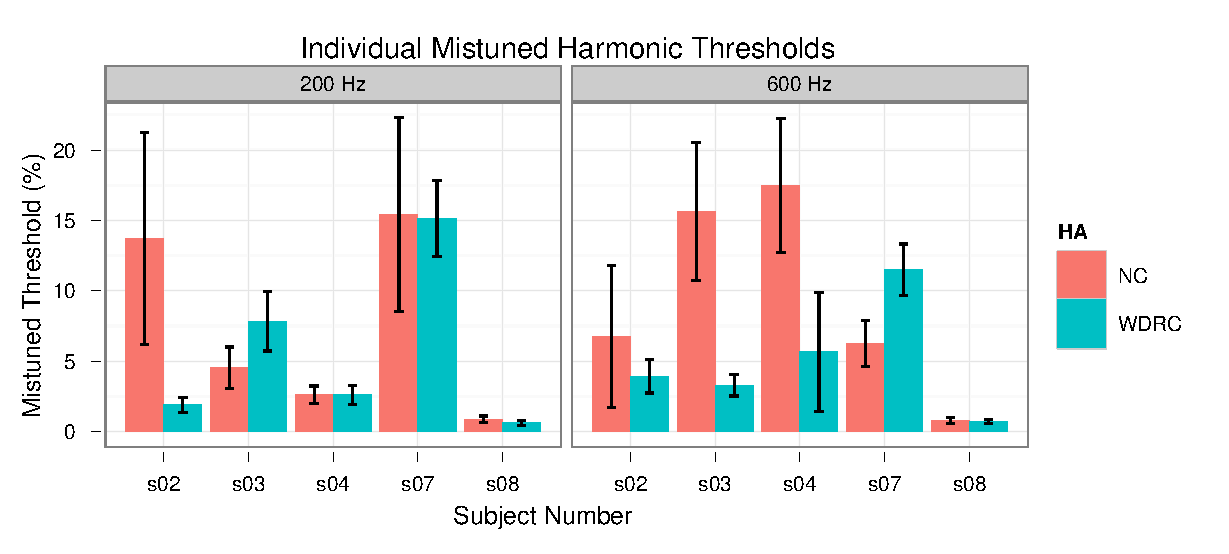
\includegraphics[height=3in]{chap4-mhn-indiv.pdf} \\
\caption[NCStudy1 mistuned harmonic - individual thresholds]{NCStudy1 mistuned harmonic - individual thresholds.  Error bars represent $\pm$ 1 SD.  There are huge individual differences on this task.}
\label{ch4-mhn-indiv}
\end{center}
\end{figure}


\subsection{Timbre Perception}
\subsubsection{Stimuli}
\paragraph{}A real recording of a tenor saxophone extracted from the Real World Computing (RWC) Music Database \cite{Goto2003} was used as the stimulus for the experiment.  The saxophone recording is of one note (F5), sounding for a duration of 953 ms.  The sound was calibrated to a presentation level of 65 dB SPL.  In order to prevent entrainment, the stimulus was played in the presence of white Gaussian noise at a SNR of +20 (the noise was measured to be 45 dB(A)).
\subsubsection{Procedure}
\paragraph{}A three-alternative forced-choice (3AFC) adaptive staircase design \cite{Levitt1971} with a 2-down, 1-up rule was used to estimate the threshold for detecting a change in timbre.  A trial consisted of 3 presentations of the saxophone stimulus (zero-padded to be 1000 ms in length) with an inter-stimulus interval (ISI) of 1000 ms.  One of the saxophone notes in a trial had one of its harmonics altered in intensity, beginning by it being completely removed, and it was the task of the participant to identify ``which saxophone note sounded different than the other two'' by selecting the corresponding button on a touchscreen.  Altering the intensity of a single harmonic changes the overall level of the instrument, and to compensate for this alteration the power of all other harmonics were multiplied by a constant to equate acoustic power across all three note presentations.

There were two blocks in the experiment, and the blocks differed with respect to the harmonic that was altered.  The first block altered the fundamental, and the second block altered the second harmonic.  These harmonics were chosen as they had the most acoustic power and therefore allowed for the most attenuation.  Each block consisted of 12 reversals (defined as a transition from at least 2 correct responses to an incorrect response, or vice versa).  Intensity was altered by an additive 20\% according to the 2-down, 1-up rule, and once 4 reversals had occurred, the percentage intensity step size was changed to 10\%.  The harmonic intensity threshold for a given block was computed by averaging the thresholds measured at the last 8 reversals in the block.

Continuous white Gaussian noise played throughout the presentation of the saxophone notes, including a 1000 ms segment before the first note and a 1000 ms segment after the last note.  The white Gaussian noise was ramped with a linear rise/fall time of 10 ms.

Feedback on performance (correct or incorrect) was given to participants on every trial via the touchscreen, and was displayed for 2000 ms.  Following the feedback, there was a silent period for 1000 ms preceding the onset of the next trial.  A practice session featuring 6 trials was included before the first experimental block to ensure that the participant understood the instructions.  The practice session was repeated until participants admitted that they understood the task, and until they exceeded 50\% correct on the practice trials.  For the vast majority of subjects, only 1 practice session was required.
\subsubsection{Results}
\paragraph{}A within-subjects ANOVA was performed, with two within-subjects factors, hearing aid (WDRC or NC), and harmonic (fundamental or second harmonic).  The dependent measure was the harmonic intensity threshold.  The only significant effect was a main effect of harmonic (F(1,4) = 39.96, p = 0.003), such that participants were more sensitive to changes in intensity of the fundamental than the second harmonic.  Though, there was a trending main effect of hearing aid (F(1,4) = 6.16, p = 0.068), such that participants tended to perform better with NC than WDRC.  Detailed statistical results may be seen in Table 4.4.  Group means and standard errors are plotted in Figure 4.16, and individual means and standard deviations are plotted in Figure 4.17.

\begin{table}[htp]
\begin{center}
\begin{tabular}{lrrrrrrrr}
       Effect & DFn & DFd  &  SSn &  SSd  &    F  &     p & p<.05  &   ges
       \\
       \hline
          HA &  1 &  4 &   446 & 289 &  6.16 & 0.068  &   .  & 0.146 \\
        harm  & 1 &  4 &  1684 & 169 & 39.96 & 0.003  &   ** & 0.392 \\
     HA:harm &  1 &  4 &     5 & 1019 &  0.02 & 0.901 &     & 0.002 \\
     \hline
\end{tabular}
\end{center}
\caption{Timbre Perception Within-Subjects Factorial ANOVA}
\end{table}

\begin{figure}[htp]
\begin{center}
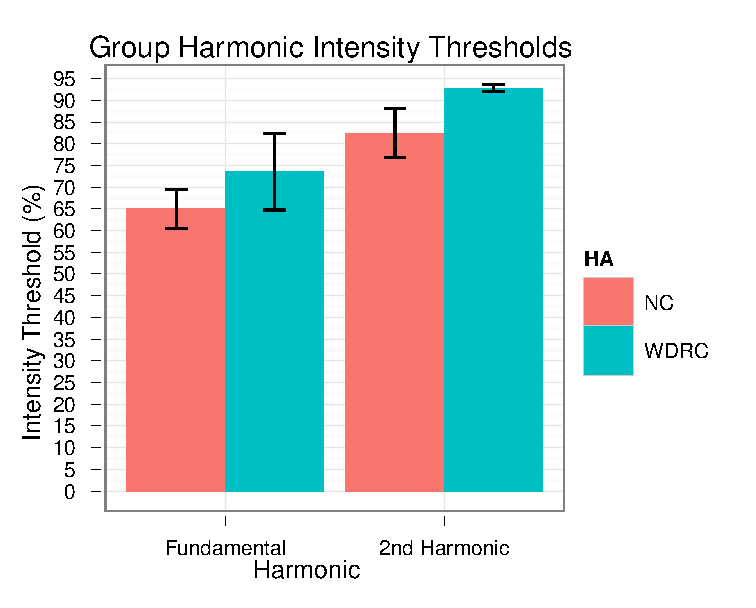
\includegraphics[height=3in]{chap4-timbre-group.pdf} \\
\caption[NCStudy1 timbre perception - group thresholds]{NCStudy1 timbre perception - group thresholds.  Error bars represent $\pm$ 1 SEM.  Participants tended to more accurately discriminate changes in timbre with the NC (F(1,4) = 6.16, p = 0.068), and intensity changes to the fundamental were easier to discriminate than changes to the second harmonic (F(1,4) = 39.96, p = 0.003).}
\label{ch4-timbre-group}
\end{center}
\end{figure}

\begin{figure}[htp]
\begin{center}
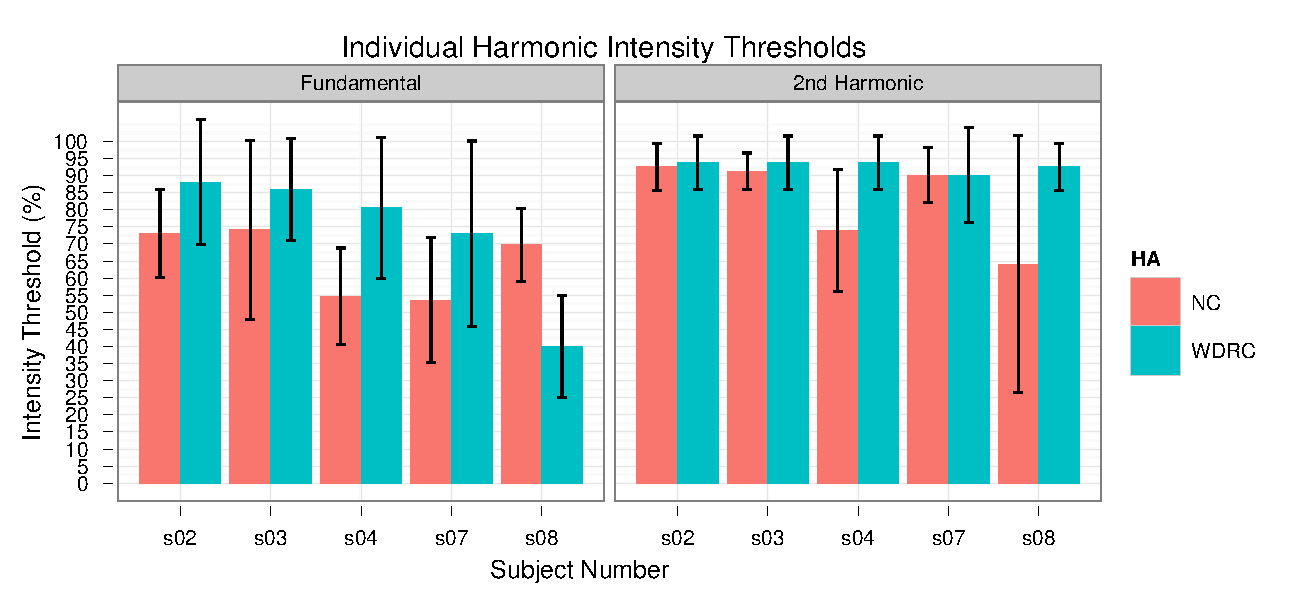
\includegraphics[height=3in]{chap4-timbre-indiv.pdf} \\
\caption[NCStudy1 timbre perception - individual thresholds]{NCStudy1 timbre perception - individual thresholds.  Error bars represent $\pm$ 1 SD.  For all cases except the fundamental for subject 08, participants were either equally as good, or better, at discriminating intensity changes with the NC.}
\label{ch4-timbre-indiv}
\end{center}
\end{figure}

\subsection{Gap Detection}
\subsubsection{Stimuli}
\paragraph{}Noise bursts were generated in Matlab with a bandwidth of 50 Hz and a centre frequency of 1000 Hz.  The noise bursts were 500 ms, cosine ramped with a rise/fall of 10 ms, and one of the noise bursts in a trial had a silent gap in the middle.  A cosine ramp was used to gate the gap on with a time frame of 1 ms, and the same time frame for gating the gap off.  The filtering and signal processing introduced noticeable spectral splatter, which can affect detection of the gap via off-frequency listening.  To prevent off-frequency listening, the gap stimuli were presented in white Gaussian noise.  The level of the noise was set at 65 dB(A), and the level of the noise burst was 70 dB(A).
\subsubsection{Procedure}
\paragraph{}A three-alternative forced-choice (3AFC) adaptive staircase design \cite{Levitt1971} was used in conjunction with a 2-down, 1-up rule and an inter-stimulus interval (ISI) of 500 ms.  Overall, a trial was 3500 ms in length, starting with white Gaussian noise only and ending with white Gaussian noise only, with the onset of the first noise burst beginning 500 ms into the stimulus.  It was the task of the participant to determine ``which one of the three sounds sounded different from the other two'', by pressing the appropriate button on the touchscreen.

The gap started with a (maximum) duration of 100 ms, and its duration was altered by a factor of 1.4 according to the 2-down, 1-up rule, continuing on for 12 reversals.  Reversals were defined as a transition from at least 2 correct responses to an incorrect response, or vice versa.  After the fourth reversal, the factor by which the gap duration was altered changed to 1.2.

Three separate blocks were run to obtain a more accurate estimate of the gap threshold, with a self-paced break in the middle of each block.  Feedback on performance (correct or incorrect) was given to participants on every trial via the touchscreen, and was displayed for 2000 ms.  Following the feedback, there was a silent period for 1000 ms preceding the onset of the next trial.  The gap detection threshold for a given block was computed by averaging together the last 8 reversals in the block.

A practice session featuring 6 trials was included before the first experimental block to ensure that the participant understood the instructions.  The practice session was repeated until participants admitted that they understood the task, and until they exceeded 50\% correct on the practice trials.  For the vast majority of subjects, only 1 practice session was required.
\subsubsection{Results}
\paragraph{}A within-subjects ANOVA was performed with hearing aid type as the only factor.  The three thresholds measured during a session (one per block) were averaged together to obtain an average threshold for that session.  In the end, there was no significant effect of hearing aid type (F(1,4) = 0.065, p = 0.812), indicating that neither hearing aid conferred a temporal processing advantage.  Group means and standard errors are plotted in Figure 4.18, and individual means and standard deviations are plotted in Figure 4.19.

\begin{figure}[htp]
\begin{center}
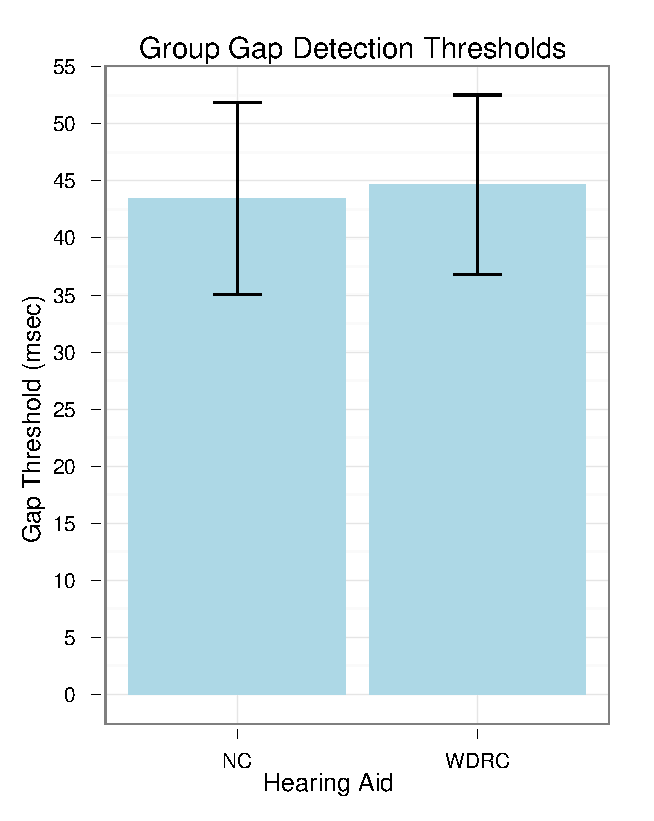
\includegraphics[height=3in]{chap4-gd-group.pdf} \\
\caption[NCStudy1 gap detection - group thresholds]{NCStudy1 gap detection - group thresholds.  Error bars represent $\pm$ 1 SEM.  There was no significant difference in performance between the hearing aid types (F(1,4) = 0.065, p = 0.812).}
\label{ch4-gd-group}
\end{center}
\end{figure}

\begin{figure}[htp]
\begin{center}
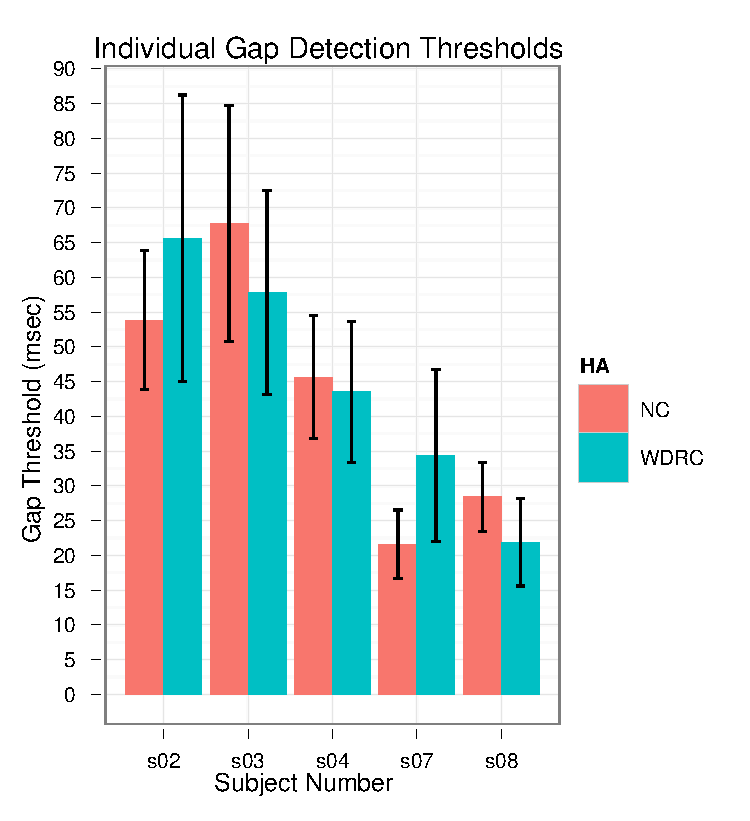
\includegraphics[height=3in]{chap4-gd-indiv.pdf} \\
\caption[NCStudy1 gap detection - individual thresholds]{NCStudy1 gap detection - individual thresholds.  Error bars represent $\pm$ 1 SD.  There were some individuals who performed better with WDRC, while others did better with NC.}
\label{ch4-gd-indiv}
\end{center}
\end{figure}

\section{Sound Localization}
\subsection{Horizontal Localization}
\subsubsection{Stimuli}
\paragraph{}The stimuli used in this experiment were similar to those used in \citeA{VandenBogaert2006}.  One-third octave noise bands centred at 500 Hz (low-frequency) and 3000 Hz (high frequency) with a duration of 200 ms were created in Matlab.  The first 50 ms and the last 50 ms of the stimuli were cosine windowed to provide a gradual rise and fall in intensity.  Both a low frequency and a high frequency condition were used to test the preservation of ITD and ILD cues by the hearing aids, respectively.  Additionally, a broadband, telephone sample was included in a separate condition to test more realistic sound localization.  The telephone stimulus was 1000 ms in duration, and contained peaks in its spectrum both in the low frequency range (less than 1500 Hz) and the high frequency range (greater than 1500 Hz), so it contained both ITD and ILD cues.
\subsubsection{Procedure}
\paragraph{}This task took 25 minutes to complete.  Both the experimenter and the participant sat in the sound attenuating chamber, with the participant seated 1.5 meters away from an array of 7 speakers suspended in a 90$^\circ$ arc (15$^\circ$ separation between speakers).  Participants were tested at two different orientations (one facing the leftmost speaker, and the other facing the rightmost speaker, in order to test both left and right hemi-fields).

The stimuli were all presented at 65 dB SPL, measured at the head of the participant.  Presentation order was completely random, and four trials of each stimulus were presented at every speaker in each condition, for a total of 168 trials per session (7 speakers * 4 trials * 3 stimulus types * 2 orientations).  There were 6 blocks of trials (3 stimulus types * 2 orientations) and the presentation order of these blocks were fixed to provide a more controlled comparison of the NC and WDRC technologies.  Adopting ``left'' and ``right'' as terminology for facing the leftmost and rightmost speakers respectively, the order of conditions in the experiment was phone-right, low-right, high-right, phone-left, low-left, high-left.

Following each stimulus presentation, the participant indicated with a laser pointer which loudspeaker they thought the sound came from by pointing at a speaker labelled from A-G in the speaker arc.  The experimenter coded the subject's response, and wore sound-isolating headphones (ANSI S3.19 Workhorse) to prevent him/her from biasing the subject's response. Subjects were instructed to remain facing straight for the duration of the experiment, rested their chin on a chin rest while sounds were playing, and were encouraged at the outset of the experiment to disengage from the chin rest if they liked, only when making their response (and after cessation of the stimulus).

A practice session consisting of 3 trials (the low frequency stimulus) was delivered before starting the phone-right condition, presenting first ``to the speaker directly in front of'' the subject, then ``to the speaker to the far left'', and finally ``to a speaker somewhere in the middle.''
\subsubsection{Results}
\paragraph{}A within-subjects ANOVA was performed, with three within-subjects factors, hearing aid (WDRC or NC), stimulus (low freq, high freq, or phone), and angle (0 to 90 $^\circ$ in 15 $^\circ$ increments).  There were too few subjects to test the sphericity assumption of the ANOVA, so results should be interpreted with caution.  The dependent measure was the error (|Stimulus$^\circ$ - Response$^\circ$|).  The only significant effects were a main effect of stimulus (F(2,8) = 13.71, p = 0.003), such that the high frequency stimulus was much more difficult than the phone or low frequency stimuli.  There was also a main effect of angle (F(6,24) = 6.66, p < 0.001), and an interaction of stimulus and angle (F(12,48) = 2.11, p = 0.034).  Detailed statistical results may be seen in Table 4.5.  Group means and standard errors are plotted, as a function of stimulus in Figure 4.20, as a function of angle in Figure 4.21, and combined in Figure 4.22.  Figure 4.23 also shows the distribution of responses on each condition for both NC and WDRC.

\begin{table}[h]
\begin{tabular}{lrrrrrrrr}
\hline
ANOVA & & & & & & & & \\
         Effect & DFn & DFd  &    SSn &  SSd   &     F   &  p & p<.05  &  ges \\
            HA &  1 &  4 &   3 & 778 & 0.02 & 0.903  &     & 0.000 \\
          stim &  2 &  8 & 3312 & 966 & 13.71 & 0.003 &    ** & 0.277 \\
         angle &  6 & 24 & 5235 & 3144 & 6.66 & 0.000 &    *** & 0.377 \\
       HA:stim &  2 &  8 & 107 & 588 & 0.73 & 0.513   &    & 0.012 \\
      HA:angle &  6 & 24 & 158 & 645 & 0.98 & 0.463   &    & 0.018 \\
    stim:angle & 12 & 48 & 783 & 1484 & 2.11 & 0.034  &   * & 0.083 \\
 HA:stim:angle & 12 & 48 & 156 & 1034 & 0.60 & 0.828  &    & 0.018 \\
\hline
\end{tabular}
\caption{Sound Localization Within-Subjects ANOVA}
\end{table}

\begin{figure}[htp]
\begin{center}
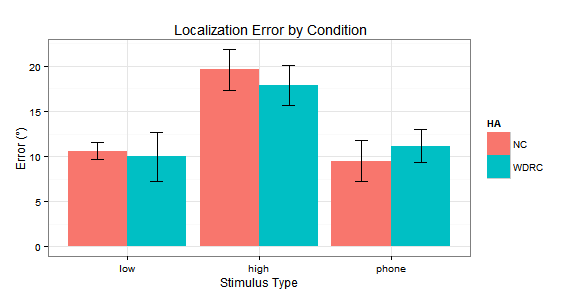
\includegraphics[height=3in]{chap4-loc-cond.png} \\
\caption[NCStudy1 sound localization results - stimulus type]{NCStudy1 sound localization results - stimulus type.  Error bars represent $\pm$ 1 SEM.  There was no significant difference between NC and WDRC (F(1,4) = 0.02, p = 0.903), but there was a main effect of stimulus (F(2,8) = 13.71, p = 0.003), such that the higher frequency sound was more difficult to localize.}
\label{chap4-loc-cond}
\end{center}
\end{figure}

\begin{figure}[htp]
\begin{center}
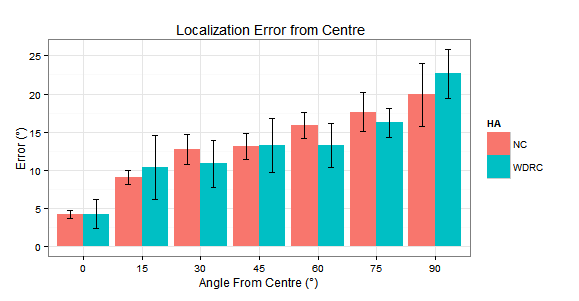
\includegraphics[height=3in]{chap4-loc-spk.png} \\
\caption[NCStudy1 sound localization results - angle]{NCStudy1 sound localization results - angle.  Error bars represent $\pm$ 1 SEM.  There was a main effect of angle (F(6,24) = 6.66, p < 0.001).  Generally speaking, the further the stimulus is presented from centre, the greater the error.}
\label{chap4-loc-spk}
\end{center}
\end{figure}

\begin{figure}[htp]
\begin{center}
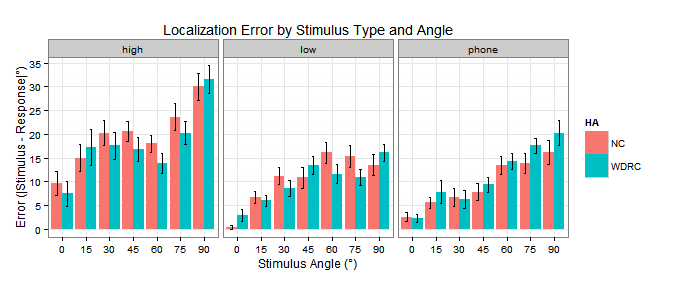
\includegraphics[height=3in]{chap4-loc-cond+spk.png} \\
\caption[NCStudy1 sound localization results - stimulus type and angle]{NCStudy1 sound localization results - stimulus type and angle.  Error bars represent $\pm$ 1 SEM.}
\label{chap4-loc-cond-spk}
\end{center}
\end{figure}

\begin{figure}[htp]
\begin{center}
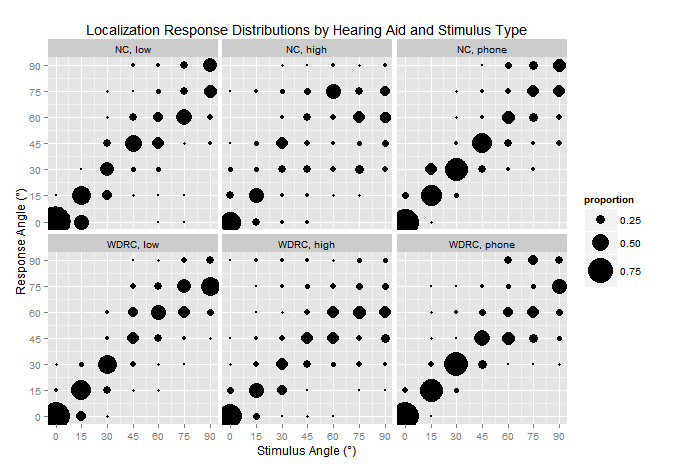
\includegraphics[height=4in]{chap4-loc-prop.png} \\
\caption[NCStudy1 sound localization results - response distributions]{NCStudy1 sound localization response distributions.  Circle area is proportional to number of responses at a particular stimulus, response configuration.}
\label{chap4-loc-cond-prop}
\end{center}
\end{figure}

\section{Subjective Measures}
\subsection{Abbreviated Profile of Hearing Aid Benefit (APHAB)}
\subsubsection{Procedure}
\paragraph{}To compare the NC and WDRC using this inventory, we administered the APHAB as the very last task during the second test session for both the NC and WDRC trial periods.  Completion of this inventory took approximately 10 minutes.
\subsubsection{Results}
\paragraph{}There was no easy way of looking at group results for the APHAB, because the APHAB software outputs an unaided and aided graph for each subject, as opposed to raw data.  APHAB results are reported for NCStudy2, but they were too difficult to tabulate for NCStudy1.

\subsection{Sound Quality}
\subsubsection{Procedure}
\paragraph{}The sound quality questionnaire was administered to assess dimensions of music quality on a 5 point scale (fullness, naturalness, pleasantness, clarity), and a final composite score was computed by averaging the scores on these scales together.  The overall sound quality component of the questionnaire asked participants to rate how pleasant/unpleasant sound was for a variety of situations (a talker in quiet, car radio, etc.).  The questionnaire is attached in the Appendix.

The questionnaire was administered during the second test session for each hearing aid trial period.

\subsubsection{Results}
\paragraph{}A within-subjects ANOVA was performed, with two within-subjects factors, hearing aid (WDRC or NC), and questionnaire subtype (music or overall).  The dependent measure was a composite score of sound quality, computed by averaging sound quality scores across each questionnaire subtype.  The only significant effect was a main effect of questionnaire subtype (F(1,4) = 15.42, p = 0.017).  Detailed statistical results may be seen in Table 4.6.  Group means and standard errors are plotted in Figure 4.24.

\begin{figure}[htp]
\begin{center}
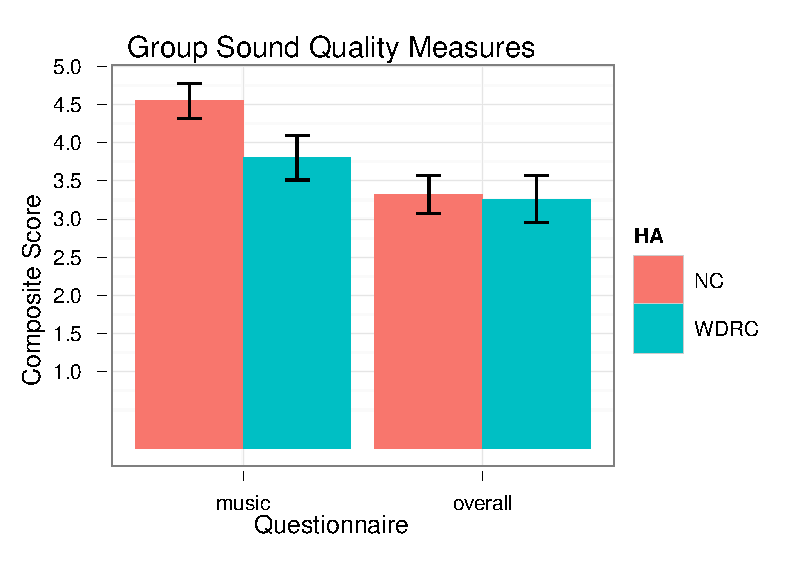
\includegraphics[height=3in]{chap4-sound-qual-group.pdf} \\
\caption[NCStudy1 sound quality group results]{NCStudy1 sound quality group results.  Error bars represent $\pm$ 1 SEM.  There was no significant main effect of hearing aid (F(1,4) = 1.16, p = 0.342).}
\label{ch4-sound-qual-group}
\end{center}
\end{figure}

\subsection{Feedback Form}
\subsubsection{Results}
\paragraph{}Participants were given a questionnaire at the very end of the study, asking them to report which set of hearing aids they preferred for a variety of listening situations, and to give an overall preference of hearing aid type.  Table 4.6 presents the number of participants who preferred NC and WDRC for each listening situation.

\begin{table}[htp]
\centering
\begin{tabular}{lrrrrr}
  \hline
  Situation & NC Count & WDRC Count \\
  \hline
  Music        & 4 & 1 \\
  Speech in quiet & 4 & 1 \\
  Speech in noise & 3.5 & 1.5 \\
  Television & 3 & 2 \\
  Telephone & 4.5 & 0.5 \\
  Overall & 3.5 & 1.5 \\
   \hline
\end{tabular}
\caption{Listening Situation Preferences}
\end{table}

\section{Discussion}
\paragraph{}In this section, the results of the present experiment are synthesized as best as possible.  However, there were several limitations in the study design, which prevents the conclusions from being maximally meaningful.  First, the study limitations will be discussed, followed by a synopsis of results in each auditory domain, so that the reader may interpret the conclusions drawn from each auditory domain with the study limitations in mind.

\subsection{Limitations}
\paragraph{}First, it is uncertain as to how much amplification was being delivered by the NC and WDRC hearing aids as a function of frequency, since real ear measurements were not performed.  Although the fitting software offered by hearing aid manufacturers allows clinicians to see the amount of amplification given by hearing aids, these visualizations are not always completely accurate \cite{Hawkins2003}.  Real ear measurements offer a method that clinicians can use to verify the amount of gain given by a hearing aid.  In the real ear measurement procedure, a tiny probe microphone is placed in a participant's ear close to the tympanic membrane, and the sound level of a given stimulus (usually some sort of speech shaped noise) is measured with the hearing aid in the participant's ear, and without the hearing aid in the participant's ear.  By calculating the difference between these two values, a measure of real-ear insertion gain is computed.  Not knowing the gain provided by each hearing aid type is a problem, because if one hearing aid type was consistently delivering more gain than the other, it could have made the test stimuli more audible for one hearing aid type, potentially biasing performance on many of the psychoacoustic tasks.

Second, the NC and WDRC hearing aids differed in many respects, such as the age of the hearing instruments, the quantity and quality of adjustments that the hearing aids received, and the features programmed onto the hearing aids.  The WDRC hearing aids were much older than the NC hearing aids, so it is possible that the NC hearing aids had newer processors and electrical components which could have influenced task performance.  On the other hand, participants had had several adjustments performed on their WDRC hearing aids, so hearing aid fittings could have been more fine-tuned for the WDRC hearing aids.  One other complication is that the specialist fine-tuning the NC aids was not the same specialist as those that participants worked with to fine-tune their own WDRC hearing aids.  There was no way to control for specialist skill in the current study.  One last major difference between the NC and WDRC hearing aids were the features that were programmed onto the hearing aids.  The NC hearing aids were programmed with 2 programs: program 1 had feedback cancellation only, and program 2 had feedback cancellation and directional microphones to help with speech in noise in everyday environments.  Most of the WDRC hearing aids had automatic programs, which automatically decide when to activate features such as noise reduction, and directionality.  All of the hearing aids in the study had feedback cancellation systems, and most of the WDRC hearing aids had noise reduction enabled as well.

Third, there could be selection bias in the recruiting process for the study.  It is conceivable that out of the whole population of eligible participants for the study (all hearing aid users with 2 functioning hearing aids, with symmetric sensorineural hearing loss), there may have been a tendency for those who were dissatisfied with their current WDRC hearing aids to sign up to participate in the study.  Alternatively, the reverse could be true.  Perhaps those who are satisfied with their current hearing aids would be more open to try new hearing aids, due to positive prior experiences with hearing aids.

Fourth, there could have been adaptation effects contaminating the data.  There are data which suggest that it can take an extended period of time to adapt to a hearing aid fitting \cite{Brooks1996}.  The adaptation period for the NC may not have been long enough, limiting the NC's effectiveness.  Despite asking participants at the outset of the study to wear the hearing aids as much as possible during the course of the study, there was also no way of knowing how often participants were wearing the hearing aids on a daily basis.  Certainly, participants would not have adapted as well to the NC hearing aids had they not worn the hearing aids consistently throughout the trial period.  An added complication related to this, is that the WDRC hearing aids were always accessible to participants (we could not confiscate the participants' own hearing aids), whereas the NC hearing aids were only accessible during the portion of the study for which they were wearing the NC hearing aids.

Fifth, the hearing aids were programmed on old audiograms for 3 of the participants, and for 2 of the participants only the new audiograms could be used to program the hearing aids.  Programming the hearing aids on the old audiograms could have potentially compromised the NC training algorithm, which expects correct audiogram data.  However, using newer audiograms to program the NC for 2 participants could have biased the performance of these individuals in favor of the NC.

\subsection{Conclusions from NCStudy1}
\paragraph{}NCStudy1 was confounded with too many variables that were outside of the experimenter's control, making any interpretation of the results quite difficult.  Instead, a summary of results on each auditory domain is presented here.  Results from NCStudy1 and NCStudy2 will be synthesized and compared in the following chapters.

\subsubsection{Speech Intelligibility}
\paragraph{}There were fairly consistent differences between the NC and WDRC hearing aids in terms of individual phonemes correctly recognized.  The NC was not as good at restoring particular consonants, such as /b/, /h/, and /r/.  Vowel recognition was more equal between hearing aids; there was a tendency for /who'd/ to be restored better with the NC, while recognition of /hayed/ was superior with WDRC.  These differences are unlikely to be due to any effect of noise reduction enabled in WDRC but not NC, since the differences were present in both the quiet and noise conditions.

It would be premature to read too much into these results, because of the many confounds outlined in the Limitations section, above.  The real test is whether these results are replicated in NCStudy2. An important point is that despite consistent differences between the NC and WDRC hearing aids on the recognition of individual phonemes, one hearing aid did not outperform the other on a more realistic speech in noise test.

\subsubsection{Music Perception}
\paragraph{}There was no difference in temporal perception between WDRC and the NC as determined by the gap detection task, and no difference in frequency resolution as determined by the mistuned harmonic task.  There was, however, a trend for better intensity resolution of particular harmonics for the NC hearing aid.

Again, these results should be interpreted with caution.  It would be overly simple to claim that the NC restores timbre perception due to it restoring a more normal neural signal at the level of the auditory periphery.  To test this hypothesis, an analysis would be incomplete without computing neurograms for the saxophone stimulus, both for an impaired ear preprocessed by the NC and WDRC.  If the result holds, there are other potential reasons for why the NC was superior for timbre perception.  One potential reason is that the NC, due to its gain function, enhances frequency channels with high acoustic power, and attenuates frequency channels with low acoustic power.  Given that the harmonics which were altered in the timbre perception task were the harmonics in the saxophone stimulus with the greatest acoustic power, to allow for the most attenuation, it is possible that each step in intensity change was greater for the NC, making the task easier from trial to trial.  Another possible difference between the hearing aids which could account for performance is compression.  If WDRC was applying a greater amount of compression than NC in a given frequency channel, then the step in intensity change would have been greater for the NC.  One last possibility is that although participants did not complain of entrainment or feedback being present in any of the music perception tasks (reporting an additional tone, or a whistling), it is possible that feedback/entrainment could have contaminated results for particular subjects, affecting one set of hearing aids more than the other.

\subsubsection{Sound Localization}
\paragraph{}There were no statistically significant differences between the NC and WDRC hearing aids for sound localization.  However, the localization error by stimulus type and angle, as well as the response distributions by hearing aid and stimulus type, seems to show some trend of worse localization performance by the NC for high frequency sounds.  Perhaps not enough gain was given to high frequency sounds for the NC.  It is difficult to draw any conclusions here, given the many limitations of the present study, noted above.

\subsubsection{Subjective Measures}
\paragraph{}There were no differences between the NC and WDRC on the sound quality measure.  However, the feedback form at the end of the study seemed to indicate that participants preferred the NC overall.  This feedback form was vulnerable to demand characteristics; the study was not double-blind, so participants could have reported a preference for the NC simply to please the experimenter. 